\subsection{Lüftung}\label{sec: Lüftung}
\begin{figure}[H]
    \centering
    \includegraphics[scale=0.7]{image/arduino lüftung.png}
    \caption{Arduino Lüftungssteuerung (Verkabelung)\autocite{SchaltungLüfter}}
    \label{fig:enter-label}
\end{figure}
\vspace{3mm}
Das Bild zeigt ein elektronisches Schaltbild, in dem ein Arduino\autocite{Arduino} Board verwendet wird, um einen Lüfter zu steuern. Den Arduino habe ich nur verwendet, um die Funktion zu testen.\\
\vspace{3mm}
Der Arduino ist mit einer 12V-Stromversorgung verbunden, welche für die Versorgung des Lüfters verwendet wird. Da der Arduino mit einer Versorgungsspannung von 5V arbeitet habe ich einen NPN-Transistor verwendet, der als Schalter dient und von einem digitalen Pin des Arduinos gesteuert werden kann. \\
\vspace{3mm}
Darüber hinaus verwende ich in der Schaltung auch einen 220 Ohm Widerstand, der den Strom begrenzt und von einem digitalen Pin des Arduino bzw. des Raspberry Pi zur Basis des Transistors fließt. Das schützt den Mikrocontroller Pin vor Überlastung. \\
\vspace{3mm}
Die Schaltung wurde im ersten Schritt auf dem Steckboard aufgebaut und mit dem Arduino getestet. Danach wurde diese Schaltung auf einer Streifenrasterplatine aufgebaut und wieder getestet.\\

\subsubsection{Pinbelegung des BC547}
\begin{table}[H]
	\centering
	\begin{tabular}{ | c | c | c | } 
		\hline
		\textbf{Pin} & \textbf{Name} &\textbf{Symbol}\\ 
		\hline
		1 & Kollektor & C\\ 
		\hline
		2 & Basis& B\\ 
		\hline
		3 & Emitter & E \\ 
		\hline
	\end{tabular}
	\caption{Stückliste Pneumatik}
\end{table}
\vspace{2mm}
\begin{figure}[H]
	\centering
	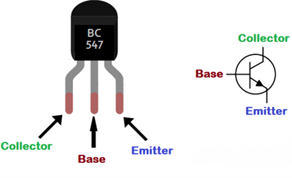
\includegraphics{image/pinbelegung transistor.png}
	\caption{Pinbelegung des BC547-Transistor\autocite{BC547Bild}}
	\label{fig:enter-label}
\end{figure}
Abbildung 60 zeigt die symbolische Pinbelegung des Transistors (BC547) als Bauteil und als Schaltsymbol. Der Transistor hat drei Anschlüsse: Basis (B), Kollektor (C) und Emitter (E). Die Basis ist der Steueranschluss, über den der Fluss der Elektronen zwischen Emitter und Kollektor gesteuert wird.

\newpage
\subsubsection{Aufbau Lüfter}
\begin{figure}[H]
    \centering
    \includegraphics[scale = 0.7]{image/lüfterstreifen.png}
    \caption{Aufbau Streifenrasterplatine (Lüftungssteuerung)}
    \label{fig:enter-label}
\end{figure}
\vspace{3mm}
Die Abbildung zeigt den Aufbau für die Lüftungssteuerung mittels Streifenrasterplatine. 

\subsubsection{Befestigung}
\begin{figwindow}[0,r,\includegraphics[scale=0.6]{image/befestigunglüfter.jpg},{Lüfter am Plexiglas}]
Das Plexiglas hat die Maße 72cm x 22,5cm und der Lüfter hat die Maße 12cm x 12cm. \\

Der Lüfter muss in der Mitte des Plexiglases befestigt werden. Für die mechanische Befestigung des Lüfters am Plexiglas sind vier Löcher vorgesehen.\\

Danach wird eine Bohrung im Mittelpunkt gemacht, damit man später den Durchmesser des Lüfters ausschneiden kann.
\end{figwindow}